\documentclass[12pt, A4]{report}

\usepackage{amsmath}
\usepackage{amssymb}
\usepackage{bm}
\usepackage{fancyhdr}
\usepackage{hyperref}
\usepackage[margin=0.75in]{geometry}
\usepackage[utf8]{inputenc}
\usepackage{tikz}
\usetikzlibrary{calc}

% Configuration
\title{AP Calculus Practice Problems}
\author{Arnav Patri}

\pagestyle{fancy}
\fancyhf{}
	\fancyhead[L]{\leftmark}
	\fancyhead[R]{Arnav Patri}
	\fancyhead[C]{\thepage}
	\fancyfoot{}
	\renewcommand{\chaptermark}[1]{\markboth{#1}{}}

% Symbols
\renewcommand{\d}{\text{d}}

\begin{document}
	\chapter*{Volume: Disk/Washer\markboth{Volume: Disk/Washer}{}}
		Arnav Patri
		\section*{Sources}
			\subsection*{Calculus: Early Transcendentals 9$^{\textbf{th}}$ Edition}
				\begin{enumerate}
					\setcounter{enumi}{1}
					\item
						6.2 Exercise 12
						\setcounter{enumi}{3}
					\item
						6.2 Exercise 15
					\item 
						6.2 Exercise 1
						\setcounter{enumi}{6}
					\item
						6.2 Exercise 17
						\setcounter{enumi}{7}
					\item
						6.2 Exercise 24
				\end{enumerate}
			\subsection*{\href{https://www.youtube.com/watch?v=BcFEcRimurc}{Calculus 2: Washer Method (HARD Problems}) by Ludus}
				\qquad \href{https://www.youtube.com/watch?v=BcFEcRimurc}{https://www.youtube.com/watch?v=BcFEcRimurc}
				\begin{enumerate}
					\setcounter{enumi}{5}
					\item
						Example 1
						\setcounter{enumi}{7}
					\item
						Example 2
				\end{enumerate}
			\subsection*{AP Calculus Exams}
				\begin{enumerate}
					\setcounter{enumi}{10}
					\item
						2021 AB FRQ 3(c)
				\end{enumerate}
			\newpage
		\section*{Problems}
			If no instructions are given, evaluate the volume of the solid generated by revolving the region bounded by the given equations about the specified line using the disk/washer method.
			\begin{enumerate}
				\item
					\[
						\left.\begin{aligned}
							y &= r &
								y &= 0 \\
							x &= 0 & 
								x &= h
						\end{aligned}\,\right|\, y = 0
					\]
				\item
					\[
						\left.\begin{aligned}
							y &= 0 &
								y &= \frac{1}{x} \\
							x &= 1 &
								x &= 4
						\end{aligned}\,\right|\, 
						\begin{aligned}
 							y &= 0
 						\end{aligned}
					\]
				\item
					\[
						\left.\begin{aligned}
							y &= 0 & 
								y &= \frac{1}{\sqrt{1 + x^2}} \\
							x &= 0 
						\end{aligned}\right| y = 0
					\]
				\item
					\[
						\left.\begin{aligned}
							y &= \frac{x^2}{4} &
								y &= 9 \\
							x &= 0
						\end{aligned}\,\right|\, x = 0
					\]
				\item
					\[
						\left.\begin{aligned}
							y &= 0 & 
								y &= x^2 + 5 \\
							x &= 0 &
								x &= 3
						\end{aligned}\,\right|\, y = 0
					\]
				\item
					\[
						\left.\begin{aligned}
							y &= 1 + \sec x &
								y &= 3 \\
							1 + \sec x &\le 3 &
								-\frac{\pi}{2} &\le x \le \frac{\pi}{2}
						\end{aligned}\,\right|\, y = 1
					\]
				\item
					\[
						\left.\begin{aligned}
							y &= x^2 &
							y &= 2x \\
						\end{aligned}\,\right|\, x = 0
					\]
				\item
					\[
						\left.\begin{aligned}
							x &= y^2 &
								x &= 1 - y^2 \\
						\end{aligned}\,\right|\, x = 3
					\]
				\item
					\[
						\left.\begin{aligned}
							y &= x^2 - 2x &
								y &= x \\
						\end{aligned}\,\right|\, y = 4
					\]
				\item
					\[
						\left.\begin{aligned}
							y &= \sin x &
								y &= \cos x \\
							x &\ge 0 & 
								x &\le \frac{\pi}{4}
						\end{aligned}\,\right|\, y = -1
					\]
				\item
					\[f(x) = cx\sqrt{4 - x^2}\]
					The solid of revolution generated by rotating the area bounded by $f$ and the $x$-axis in the first quadrant about the $x$-axis is equal to $2\pi$. Solve for $c$, given that it is a positive constant.
				\item
					\[
						\left.\begin{aligned}
							x &= (y - k)^2 &
								y &= x + k \mid k \le 0 \text{ or } k \ge 1 \\
						\end{aligned}\,\right|\, x = k
					\]
				\item
					\[
						\left.\begin{aligned}
							\frac{x^2}{a^2} - \frac{y^2}{b^2} &= 1 \mid a, b \ne 0 &
								x &= \left|\frac{ay}{b}\right| \\
							x &= a^2 &
								x &= \sqrt{a^2 + b^2}
						\end{aligned}\,\right|\, x = 0
					\]
				\item
				\[
					\left.\begin{aligned}
						\frac{x^4}{a^2} - \frac{y^2}{b^2} &= 1 \mid a, b \ne 0 &
							x^2 &= \frac{ay}{b} \\
						y &= 0 &
							y &= b
					\end{aligned}\right| x = 0
				\]
				\item
					\[
						\left.\begin{aligned}
							x^2 + y^2 &= r^2 & 
								\frac{x^2}{a^2} + \frac{y^2}{b^2} &= 1 
								\mid a, b > r > 0\\
							\text{(a) } y &= 0
						\end{aligned}\,\right|\,
						\begin{aligned}
							\text{(a) } &y = 0 \\
							\text{(b) } &y = b
						\end{aligned}
					\]
			\end{enumerate}
			\newpage
		\section*{Solutions}
			\begin{enumerate}
				\item
					\[
						V = \pi\int_0^h\left[r^2\right]\d x
								= \pi\left[r^2x\right]_0^h
								= \pi\left[r^2h - (0)\right]
								= \pi r^2h
					\]
				\item
					\[
						V = \pi\int_1^4\left(\frac{1}{x}\right)^2\d x
								 = \pi\left[-\frac{1}{x}\right]_1^4
								 = \pi\left[-\frac{1}{4} -\left(-\frac{1}{1}\right)\right]
								 = \frac{3\pi}{4} \\
					\]
				\item
					\begin{align*}
						\frac{1}{\sqrt{1 + x^2}} &= 0 \implies x \to \infty\\
						V &= \pi\int_0^\infty\left(\frac{1}{\sqrt{1 + x^2}}\right)^2\d x
								= \pi\int_0^\infty\left[\frac{1}{1 + x^2}\right]\d x
								= \pi[\arctan x]_0^{\infty}
								= \pi\left[\frac{\pi}{2} - (0)\right]
								= \frac{\pi^2}{2}
					\end{align*}
				\item
					\begin{align*}
						y &= \frac{x^2}{4} \implies x = 2\sqrt{y} \\
						y_1 &= 2\sqrt{0} = 0 \\
						V &= \pi\int_0^9\left(2\sqrt{y}\right)^2\d y = \pi\left[2y^2\right]_0^9 = 2(81)\pi = 162\pi
					\end{align*}
				\item
					\begin{align*}
						V &= \pi\int_0^3\left(x^2 + 5\right)^2\d x 
								= \pi\int_{0}^3\left[x^4 + 10x^2 + 25\right]\d x 
								= \pi\left[\frac{x^5}{5} + \frac{10x^3}{3} + 25x\right]_0^3 \\
							&= \pi\left[\frac{3^5}{5} + \frac{10(3)^3}{3} + 25(3) - (0)\right] 
								= \pi\left[\frac{243}{5} + 90 + 75\right] 
								= \frac{\pi(243 + 825)}{5} 
								= \frac{1068\pi}{5} \\
					\end{align*}
				\item
					\begin{align*}
						1 + \sec x &= 3 \implies \sec x = 2 \implies x = \pm\frac{\pi}{3} \\
						V &= \pi\int_{-\pi/3}^{\pi/3}\left[(3 - 1)^2 - (1 + \sec x - 1)^2\right]\d x
								= 2\pi\int_0^{\pi/3}\left[4 - \sec^2 x\right]\d x \\
							&= 2\pi[4x - \tan x]_0^{\pi/3} = 2\pi\left[\frac{4\pi}{3} - \sqrt{3} - (0)\right] = \frac{8\pi^2}{3} - 2\pi\sqrt{3}
					\end{align*}
				\item
					\begin{align*}
						y &= x^2 \implies x = \sqrt{y} \qquad 
								y = 2x \implies x = \frac{y}{2} \\
						\sqrt{y} &= \frac{y}{2} 
								\implies 4y = y^2 
								\implies 0 = y(y - 4) 
								\implies y_1 = 0, y_2 = 4 \\
						V &= \pi\int_0^4\left[\left(\sqrt{y}\right)^2 - \left(\frac{y}{2}\right)^2\right]\d y
							 	= \pi\int_0^4\left[y - \frac{y^2}{4}\right]\d y
							 	= \pi\left[\frac{y^2}{2} - \frac{y^3}{12}\right]_0^4 \\
							 &= \pi\left[\frac{y^2(6 - y)}{12}\right]_0^4
							 	= \pi\left[\frac{4^2(6 - 4)}{12} - (0)\right]
							 	= \pi\left[\frac{16(2)}{12}\right]
							 	= \frac{8\pi}{3}
					\end{align*}
				\item
					\begin{align*}
						y^2 &= 1 - y^2 \implies 2y^2 = 1 \implies y = \pm\frac{\sqrt{2}}{2} \\
						V &= \pi\int_{-\sqrt{2}/2}^{\sqrt{2}/2}\left[\left(y^2 - 3\right)^2 -\left(1 - y^2 - 3\right)^2\right]\d y
								= 2\pi\int_0^{\sqrt{2}/2}\left[\left(y^2 - 3\right)^2 - \left(-y^2 - 2\right)^2\right]\d y \\
							&= 2\pi\int_0^{\sqrt{2}/2}\left[y^4 - 6y^2 + 9 - \left(y^4 + 4y^2 + 4\right)\right]\d y
								= 2\pi\int_0^{\sqrt{2}/2}\left[5 - 10y^2\right]\d y \\
							&= 2\pi\left[5y - \frac{10y^3}{3}\right]_0^{\sqrt{2}/2}
								= 2\pi\left[\frac{5\sqrt{2}}{2} - \frac{10}{3}\left(\frac{\sqrt{8}}{8}\right)\right]
								= \pi\left[5\sqrt{2} - \frac{40\sqrt{2}}{24}\right]
								= \frac{10\pi\sqrt{2}}{3}
					\end{align*}
				\item
					\begin{align*}
						x &= x^2 - 2x 
								\implies 0 = x^2 - 3x = x(x - 3) 
								\implies x_1 = 0, x_2, = 3 \\
						V &= \pi\int_0^3\left[\left(x^2 - 2x - 4\right)^2 - (x - 4)^2\right]\d x \\
							&= \pi\int_0^3\left[x^4 - 2x^3 - 4x^2 - 2x^3 + 4x^2 + 8x - 4x^2 + 8x + 16 - \left(x^2 - 8x + 16\right) \right]\d x \\
							&= \pi\int_0^3\left[x^4 - 4x^3 - 4x^2 + 16x + 16 - \left(x^2 - 8x + 16\right)\right]\d x \\
							&= \pi\int_0^3\left[x^4 - 4x^3 - 5x^2 + 24x\right]\d x
								= \pi\left[\frac{x^5}{5} - x^4 - \frac{5x^3}{3} + 12x^2\right]_0^3 \\
							&= \pi\left[\frac{x^2\left(3x^3 - 15x^2 - 25x + 180\right)}{15}\right]_0^3
								= \pi\left[\frac{3(81 - 135 - 75 + 180)}{5} - (0)\right] \\
							&= \frac{3\pi(51)}{5} = \frac{153}{5}
					\end{align*}
				\item
					\begin{align*}
						\sin x &= \cos x 
								\implies x = \frac{\pi}{4} \\
						V &= \pi\int_0^{\pi/4}\left[(\cos x + 1)^2 - (\sin x + 1)^2\right]\d x \\
							&= \pi\int_0^{\pi/4}\left[\cos^2x + 2\cos x + 1 - \sin^2 x - 2\sin x - 1\right]\d x \\
							&= \pi\int_0^{\pi/4}\left[\cos(2x) + 2\cos x - 2\sin x\right]\d x
								= \pi\left[\frac{\sin(2x)}{2} + 2\sin x + 2\cos x\right]_0^{\pi/4} \\
							&= \pi\left[\frac{1}{2} + \sqrt{2} + \sqrt{2} - (0 + 0 + 2)\right]
								= \frac{(4\sqrt{2} - 3)\pi}{2}
					\end{align*}								
				\item
					\begin{align*}
						0 &= cx\sqrt{4 - x^2} \implies 
							\begin{cases}
	 							x = 0 \\
	 							\sqrt{4 - x^2} = 0 &\implies 4 - x^2 = 0 
	 								\implies 4 = x^2 
	 								\implies x = 2
							\end{cases} \\
						2\pi &= \pi\int_0^2\left(cx\sqrt{4 - x^2}\right)^2\d x
									= \pi\int_0^2\left[c^2x^2(4 - x^2)\right]\d x
									= \pi\int_0^4\left[4c^2x^2 - c^2x^4\right]\d x \\
								&= \pi\left[\frac{4c^2x^3}{3} - \frac{c^2x^5}{5}\right]_0^2
									= \pi\left[\frac{4c^2(2)^3}{3} - \frac{c^2(2)^5}{5} - (0)\right]
									= \pi\left[\frac{32c^2}{3} - \frac{32c^2}{5}\right] \\
							2 &= 32c^2\left(\frac{1}{3} - \frac{1}{5}\right) 
									= \frac{64c^2}{15} \\
							c &= \sqrt{\frac{30}{64}} = \sqrt{\frac{15}{32}}
					\end{align*}
				\item
					\begin{align*}
						y &= x + k
								\implies x = y - k \\
					\end{align*}
					For both equations, $k$ only controls a vertical shift. As this shift is the same for both equations, the area between the curves is constant regardless of the value of $k$. The volume when revolved about the same axis will therefore also be the same.
					\begin{align*}
						y &= y^2 
								\implies 0 = y(y - 1) 
								\implies y_1 = 0, y_2 = 1 \tag{$k = 0$} \\
						V &= \pi\int_0^1\left[(y - k)^2 - (y^2 - k)^2\right]\d y
								= \pi\int_0^1\left[y^2 - 2ky + k^2 - y^4 + 2ky^2 - k^2\right]\d y \\
							&= \pi\int_0^1\left[-y^4 + y^2(2k + 1) - 2ky\right]\d y
								= \pi\left[-\frac{y^5}{5} + \frac{y^3(2k + 1)}{3} - ky^2\right]_0^1 \\
							&= \pi\left[\frac{-3y^5 + 5y^3(2k + 1) - 15ky^2}{15}\right]_0^1
								= \pi\left[\frac{-3 + 5(2k + 1) - 15k}{15} - (0)\right] \\
							&= \frac{\pi(-3 + 10k + 5 - 15k)}{15} 
								= \frac{\pi(2 - 5k)}{15}
					\end{align*}
				\item
					\begin{align*}
						\frac{x^2}{a^2} - \frac{y^2}{b^2} &= 1 
									\implies x = a\sqrt{1 + \frac{y^2}{b^2}}
										= \frac{a\sqrt{b^2 + y^2}}{b} \\
							\frac{x^2}{a^2} - \frac{y^2}{b^2} &= 1 \implies y 
									= \frac{b\sqrt{x^2 - a^2}}{a} \\
							y_1 &= \frac{b\sqrt{a^4 - a^2}}{a} 
									= b\sqrt{a^2 - 1} \qquad 
								y_2 = \frac{b\sqrt{a^2 + b^2 - a^2}}{a} 
									= \frac{b^2}{a} \\
						V &= 2\pi\left|\int_{b\sqrt{a^2 - 1}}^{b^2/a}\left[\left(\frac{a\sqrt{b^2 + y^2}}{b}\right)^2 - \left(\frac{ay}{b}\right)^2\right]\d y\right|
								= 2\pi\left|\int_{b\sqrt{a^2 - 1}}^{b^2/a}\left[\frac{a^2(b^2 + y^2 - y^2)}{b^2}\right]\d y\right| \\
							&= 2\pi\left|\int_{b\sqrt{a^2 - 1}}^{b^2/a}\left[a^2\right]\d y\right|
								= 2\pi\left|\left[a^2y\right]_{b\sqrt{a^2 - 1}}^{b^2/a}\right| 
								= 2\pi\left|\frac{a^2b^2}{a} - \left(a^2b\sqrt{a^2 - 1}\right)\right| \\
							&= \left|2\pi ab\left(b - a\sqrt{a^2 - 1}\right)\right|
					\end{align*}
				\item
					\begin{align*}
						1 &= \frac{x^4}{a^2} - \frac{y^2}{b^2}
								\implies x = \sqrt{\frac{a\sqrt{b^2 + y^2}}{b}} \\
						V &= 2\pi\left|\int_0^b\left[\frac{a\sqrt{b^2 + y^2}}{b} - \frac{ay}{b}\right]\d y\right|
								= 2\pi\left|\int_0^b\left[\frac{a\left(\sqrt{b^2 + y^2} - y\right)}{b}\right]\d y\right| \\
						I(\alpha) &= \int\left[\sqrt{\alpha^2 + y^2}\right]\d y \\
						y &= \alpha\tan\theta  \implies \d y = \alpha\sec^2\theta\d\theta\\
						I(\alpha) &= \int\left[\alpha\sec^2\theta\sqrt{\alpha^2 + \alpha^2\tan^2\theta}\right]\d\theta 
								= \int\left[\alpha^2\sec^3\theta\right]\d\theta \\
						u &= \sec\theta 
								\implies \d u = \sec\theta\tan\theta 
								\qquad \d v = \sec^2\theta 
									\implies v = \tan\theta \\
						\int\left[\sec^3\theta\right]\d\theta &= uv - \int v\,\d u
								= \sec\theta\tan\theta - \int\left[\sec\theta\tan^2\right]\d\theta \\
						\int\left[\sec\theta\tan^2\theta\right]\d\theta &= \int\left[\sec\theta\left(\sec^2\theta - 1\right)\right]\d\theta
								= \int\left[\sec^3\theta - \sec\theta\right] \\
								&= \int\left[\sec^3\theta\right]\d\theta - \ln|\sec\theta + \tan\theta| \\
						\int\left[\sec^3\theta\right]\d\theta &= \sec\theta\tan\theta + \ln|\sec\theta + \tan\theta| - \int\left[\sec^3\theta\right]\d\theta \\
						2\int\left[\sec^3\theta\right]\d\theta &= \sec\theta\tan\theta + \ln|\sec\theta + \tan\theta| \\
						\int\left[\sec^3\theta\right]\d\theta &= \frac{\sec\theta\tan\theta + \ln|\sec\theta + \tan\theta|}{2} + C \\
						I(\alpha) &= \alpha^2\int\left[\sec^3\theta\right]\d\theta 
								= \frac{\alpha^2(\sec\theta\tan\theta + \ln|\sec\theta + \tan\theta|)}{2} \\
						\tan\theta &= \frac{y}{\alpha} \qquad \sec\theta = \frac{\sqrt{\alpha^2 + y^2}}{\alpha} \\
						I(\alpha) &= \frac{\alpha^2}{2}\left(\frac{y\sqrt{\alpha^2 + y^2}}{\alpha^2} + \ln\left|\frac{y + \sqrt{\alpha^2 + y^2}}{\alpha}\right|\right) \\
							&= \frac{1}{2}\left(y\sqrt{\alpha^2 + y^2} + \alpha^2\ln\left|\frac{y + \sqrt{\alpha^2 + y^2}}{\alpha}\right|\right) + C \\
						V &= \frac{2a\pi}{b}\left|\left[I(b) - \frac{y^2}{2}\right]_0^b\right| \\
							&= \frac{2a\pi}{b}\left|\left[\frac{1}{2}\left(y\sqrt{b^2 + y^2} + b^2\ln\left|\frac{y + \sqrt{b^2 + y^2}}{b}\right| - y^2\right)\right]_0^b\right| \\
							&= \frac{a\pi}{b}\left|\left[b\sqrt{2b^2} + b^2\ln\left|\frac{b + \sqrt{2b^2}}{b}\right| - b^2 - (0)\right]\right| \\
							&= \left|ab\pi\left(\sqrt{2} - 1 + \ln\left(1 + \sqrt{2}\right)\right)\right|
					\end{align*}
				\item
					\[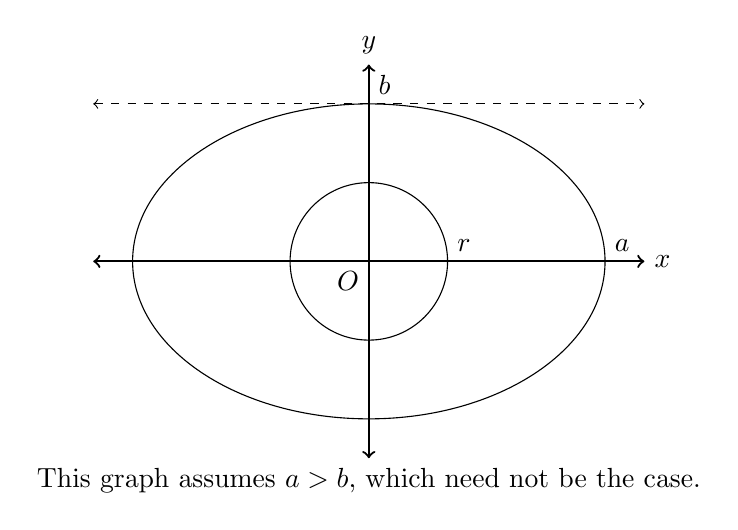
\begin{tikzpicture}
						\draw[thick, <->] (-3.5, 0) -- (3.5, 0) node[anchor = west]{$x$};
						\draw[thick, <->] (0, -2.5) -- (0, 2.5) node[anchor = south]{$y$};
							\node[anchor = north east]{$O$};
						\draw[] circle[radius = 1];
							\node[anchor = south west] at (1, 0) {$r$};
						\draw[] ellipse(3cm and 2cm);
							\node[anchor = south west] at (0, 2) {$b$};
							\node[anchor = south west] at (3, 0) {$a$};
						\draw[dashed, <->] (-3.5, 2) -- (3.5, 2);
						\node[anchor = north] at (0, -2.5) {This graph assumes $a > b$, which need not be the case.};
					\end{tikzpicture}\]
					\[
						x^2 + y^2 = r^2 
								\implies y = \sqrt{r^2 - x^2} \qquad
								\frac{x^2}{a^2} + \frac{y^2}{b^2} = 1 
									\implies y = b\sqrt{1 - \frac{x^2}{a^2}} = \frac{b\sqrt{a^2 - x^2}}{a}
					\]
					\begin{enumerate}
						\item
							\begin{align*}
								V_1 &= \pi\int_0^r\left[\left(\frac{b\sqrt{a^2 - x^2}}{a}\right)^2 - \left(\sqrt{r^2 - x^2}\right)^2\right]\d x
										= \pi\int_0^r\left[\frac{b^2(a^2 - x^2)}{a^2} - (r^2 - x^2)\right]\d x \\
									&= \pi\int_0^r\left[\frac{a^2(b^2 - r^2) + x^2(a^2 - b^2)}{a^2}\right]\d x 
										= \pi\left[\frac{a^2x(b^2 - r^2)}{a^2} + \frac{x^3(a^2 - b^2)}{3a^2}\right]_0^4 \\
									&= \pi\left[\frac{3a^2x(b^2 - r^2) + x^3(a^2 - b^2)}{3a^2}\right]_0^r
										= \pi\left[\frac{3a^2r(b^2 - r^2) + r^3(a^2 - b^2)}{3a^2}\right] \\
									&= \pi\left[\frac{3a^2b^2r - 3a^2r^3 + a^2r^3 - b^2r^3}{3a^2}\right]
										= \pi\left(\frac{3a^2b^2r - 2a^2r^3 - b^2r^3}{3a^2}\right) \\
								V_2 &= \pi\int_r^a\left(\frac{b\sqrt{a^2 - x^2}}{a}\right)^2\d x
										= \pi\int_r^a\left[\frac{b^2(a^2 - x^2)}{a^2}\right]\d x  = \pi\int_r^a\left[\frac{a^2b^2 - b^2x^2}{a^2}\right]\d x \\
									&= \pi\left[\frac{a^2b^2x}{a^2} - \frac{b^2x^3}{3a^2}\right]_r^a 
										= \pi\left[\frac{3a^2b^2x - b^2x^3}{3a^2}\right]_r^a 
										= \left[\frac{3a^3b^2 - b^2a^3}{3a^2} - \left(\frac{3a^2b^2r -b^2r^3}{3a^2}\right)\right] \\
									&= \pi\left(\frac{2a^3b^2 -3a^2b^2r + b^2r^3}{3a^2}\right) \\
								V &= 2(V_1 + V_2)
										= 2\pi\left(\frac{3a^2b^2r - 2a^2r^3 - b^2r^3 + 2a^3b^2 - 3a^2b^2r + b^2r^3}{3a^2}\right) \\
									&= 2\pi\left(\frac{2a^3b^2 - 2a^2r^3}{3a^2}\right) 
										= 4\pi\left(\frac{ab^2 - r^3}{3}\right)
							\end{align*}
						\item
 							\begin{align*}
								V_1 &= \pi\int_0^r\left[\left(\sqrt{r^2 - x^2} - b\right)^2 - \left(\frac{b\sqrt{a^2 - x^2}}{a} - b\right)^2\right]\d x \\
									&= \pi\int_0^r\left[(r^2 - x^2) - 2b\sqrt{r^2 - x^2} + b^2 - \left(\frac{b^2(a^2 - x^2)}{a^2} -\frac{2b^2\sqrt{a^2 - x^2}}{a} + b^2\right)\right]\d x \\
									&= \pi\int_0^r\left[r^2 - x^2 - 2b\sqrt{r^2 - x^2} + b^2 - b^2 +  \frac{b^2x^2}{a^2} + \frac{2b^2\sqrt{a^2 - x^2}}{a} - b^2\right]\d x \\
									&= \pi\int_0^r\left[r^2 - x^2 - 2b\sqrt{r^2 - x^2} - b^2 + \frac{b^2x^2}{a^2} + \frac{2b^2\sqrt{a^2 - x^2}}{a}\right]\d x \\
									&= \pi\left(\left[(r^2 - b^2)x + \left(\frac{b^2}{a^2} - 1 \right)\frac{x^3}{3}\right]_0^r + 2b\int_0^r\left[ \frac{b\sqrt{a^2 - x^2}}{a} - \sqrt{r^2 - x^2}\right]\d x\right) \\
								I(\alpha) &= \int\left[\sqrt{\alpha^2 - x^2}\right]\d x 
										\implies x = \alpha\sin\theta 
										\implies \d x = \alpha\cos\theta\d\theta \\
									&= \int\left[\cos\theta\sqrt{\alpha^2 - \alpha^2\sin^2\theta}\right]\d\theta
										= \int\left[\alpha^2\cos^2\theta\right]\d\theta
										= \alpha^2\int\left[\frac{\cos(2\theta) + 1}{2}\right]\d\theta \\
									&= \alpha^2\left(\frac{\sin(2\theta)}{4} + \frac{\theta}{2}\right) + C
										= \alpha^2\left(\frac{2\sin\theta\cos\theta}{4} + \frac{\theta}{2}\right) + C \\
									&= \alpha^2\left(\frac{\left(\frac{x}{\alpha}\right)\left(\frac{\sqrt{\alpha^2 - x^2}}{\alpha}\right)}{2} + \frac{\arcsin(x/\alpha)}{2}\right) + C
										= \frac{x\sqrt{\alpha^2 - x^2} + \alpha^2\arcsin(x/\alpha)}{2} + C \\
									V_1 &= \pi\left[(r^2 - b^2)x + \left(\frac{b^2}{a^2} - a\right)\frac{x^3}{3} + 2b\left(\frac{bI(a)}{a} - I(r)\right)\right]_0^r \\
										&= \begin{aligned}[t] &\pi\left[(r^2 - b^2)x + \left(\frac{b^2}{a^2} - 1 \right)\frac{x^3}{3}\right. \\ 
											&\left.+ 2b\left(\frac{bx\sqrt{a^2 - x^2} + a^2b\arcsin(x/a)}{2a} - \frac{x\sqrt{r^2 - x^2} + r^2\arcsin(x/r)}{2}\right)\right]_0^r \end{aligned} \\
										&= \begin{aligned}[t] &\pi\left[(r^2 - b^2)x + \left(\frac{b^2}{a^2} - 1 \right)\frac{x^3}{3}\right. \\ 
											&\left.+ 2b\left(\frac{xb\sqrt{a^2 - x^2} + a^2b\arcsin(x/a)}{2a} - \frac{x\sqrt{r^2 - x^2} + r^2\arcsin(x/r)}{2}\right)\right]_0^r \end{aligned} \\
										&= \begin{aligned}[t]&\pi\left[x\left(r^2 - b^2 + \frac{x^2}{3}\left(\frac{b^2}{a^2} - 1\right)\right)\right. \\ 
											&\left.+ \frac{b}{a}\left(x\left(b\sqrt{a^2 - x^2} - a\sqrt{r^2 - x^2}\right) + a^2b\arcsin\left(\frac{x}{a}\right) - r^2\arcsin\left(\frac{x}{r}\right)\right)\right]_0^r\end{aligned} \\
										&= \begin{aligned}[t]&\pi\left[r\left(r^2 - b^2 + \frac{r^2}{3}\left(\frac{b^2}{a^2} - 1\right) \right)\right. \\ 
											&\left.+ \frac{b}{a}\left(r\left(b\sqrt{a^2 - r^2} - 0\right) + a^2b\arcsin\left(\frac{r}{a}\right) - \frac{a\pi r^2}{2}\right) - (0)\right]\end{aligned}\\
										&= \pi\left(r^3 - b^2r + \frac{b^2r^3}{3a^2} - \frac{r^3}{3} + \frac{b^2r\sqrt{a^2 - r^2}}{a} + ab^2\arcsin\left(\frac{r}{a}\right) - \frac{b\pi r^2}{2}\right) \\
										&= \pi\left(\frac{2r^3(2a^2+b^2) -3a^2b\pi r^2 + 6ab^2r\left(\sqrt{a^2 - r^2} - a\right) + 6a^3b^2\arcsin(r/a)}{6a^2}\right)
							\end{align*}
							\setcounter{enumii}{1}\item (cont.)
							\begin{align*}
								V_2 &= \pi\int_r^a\left(\frac{b\sqrt{a^2 - x^2}}{a} - b\right)^2\d x
										= \pi\int_r^a\left[\frac{b^2(a^2 - x^2)}{a^2} - \frac{2b^2\sqrt{a^2 - x^2}}{a} + b^2\right]\d x \\
									&= \pi\int_r^a\left[b^2 - \frac{b^2x^2}{a^2} - \frac{2b^2\sqrt{a^2 - x^2}}{a} + b^2\right]\d x
										= \pi\int_r^a\left[2b^2 - \frac{b^2x^2}{a^2} - \frac{2b^2\sqrt{a^2 - x^2}}{a}\right]\d x \\
									&= \pi\left[2b^2x - \frac{b^2x^3}{3a^2} - \frac{2b^2I(a)}{a}\right]_r^a
										= \pi\left[2b^2x - \frac{b^2x^3}{3a^2} - \frac{b^2x\sqrt{a^2 - x^2} + a^2b^2\arcsin(x/a)}{a}\right]_r^a \\
									&= \begin{aligned}[t]&\pi\left[2b^2a - \frac{b^2a^3}{3a^2} - \frac{0 + a^2b^2(\pi/2)}{a}\right. \\
										&\left.- \left(2b^2r - \frac{b^2r^3}{3a^2} - \frac{b^2r\sqrt{a^2 - r^2} + a^2b^2\arcsin(r/a)}{a}\right)\right]\end{aligned} \\
									&= \pi\left[2ab^2 - 2b^2r + \frac{b^2r^3 - a^3b^2}{3a^2} + \frac{b^2r\sqrt{a^2 - r^2} + a^2b^2\arcsin(r/a) - 0.5a^2b^2\pi}{a}\right] \\
									&= \frac{b^2\pi\left(6a^3 - 6a^2r + r^3 - a^3 + 3ar\sqrt{a^2 - r^2} + 3a^3\arcsin(r/a) - 1.5a^3\pi\right)}{3a^2} \\
									&= \frac{b^2\pi\left(2r^3 + 6ar\left(\sqrt{a^2 - r^2} - 2a\right) + a^3(10 + 6\arcsin(r/a) - 3\pi)\right)}{6a^2} \\
								V &= 4\left(V_1 + V_2\right) \\
									&= \begin{aligned}[t]&\frac{2\pi}{3a^2}\left(4r^3(2a^2 + b^2) - 3a^2b\pi r^2 + 6ab^2r\left(2\sqrt{a^2 - r^2} - 3a\right)\right.\\
										&\left.+ a^3b^2\left(12\arcsin\left(\frac{r}{a}\right) + 10 - 3\pi\right)\right)\end{aligned}
							\end{align*}
					\end{enumerate}
			\end{enumerate}
	\chapter*{Indeterminate Exponents (Type 3)\markboth{Indeterminate Exponents}{}}
		Arnav Patri
		\section*{Sources}
			\subsection*{\href{https://www.youtube.com/watch?v=2t-E1d9_cRM}{Indeterminate Forms (Type 3)} by Faruk \"{O}zger}
				\qquad \href{https://www.youtube.com/watch?v=2t-E1d9_cRM}{https://www.youtube.com/watch?v=2t-E1d9\_cRM}
				\begin{enumerate}
					\item
						Example 2
						\setcounter{enumi}{5}
					\item
						Example 4
				\end{enumerate}
			\subsection*{Calculus: Early Transcendentals 9$^{\textbf{th}}$ Edition}
				\begin{enumerate}
					\setcounter{enumi}{2}
					\item
						4.4 Exercise 61
						\setcounter{enumi}{4}
					\item
						4.4 Exercise 57
						\setcounter{enumi}{7}
					\item
						4.4 Exercise 60
					\item
						4.4 Exercise 65
					\item
						4.4 Exercise 66
				\end{enumerate}
			\newpage
		\section*{Problems}
			Evaluate the following limits. Use comparative growth rates when necessary.
			\begin{enumerate}
				\item
					\[\lim_{x\to 0^+}\left[x^x\right]\]
				\item
					\[\lim_{x\to\infty}\left(\frac{1}{x}\right)^{1/x}\]
				\item
					\[\lim_{x\to 1^+}\left[x^{1/(1 - x)}]\right]\]
				\item
					\[\lim_{x\to\infty}(\ln x)^{1/x}\]
				\item
					\[\lim_{x\to\infty}\left(\frac{1}{e^x}\right)^{\arctan x - \pi/2}\]
				\item
					\[\lim_{x\to 0^+}\left[x^{\sqrt{x}}\right]\]
				\item
					\[\lim_{x\to 0^+}(1 + \sin(7x))^{\cot(5x)}\]
				\item
					\[\lim_{x\to\infty}\left(1 + \frac{a}{x}\right)^{bx}\]
				\item
					\[\lim_{x\to 0^+}(4x + 1)^{\cot x}\]
				\item
					\[\lim_{x\to 0^+}(1 - \cos x)^{\sin x}\]
				\item
					\[\lim_{x\to 0}\left(\frac{\sin x}{x}\right)^\frac{\cos x}{x}\]				
				\item
					\[\lim_{x\to \infty}\left(\sum_{n = 0}^\infty\left[\frac{1}{x^n}\right]\right)^x\]
				\item
					\[\lim_{n\to 1^+}\left(\int_n^\infty\left[\frac{1}{x^n}\right]\d x\right)^{n - 1}\]
				\item
					\[\lim_{n\to\infty}\left(\int_n^{\infty}\left[\frac{1}{x^n}\right]\d x\right)^{\int_{n + 1}^\infty\left[\frac{1}{x^{n + 1}}\right]\d x}\]
				\item
					\[\lim_{b\to\infty}\left(\int_0^b\left[\sum_{n = 0}^\infty\left[\frac{1}{x^n}\right]\right]\d x\right)^{e^{-b}}\]
			\end{enumerate}
			\newpage
		\section*{Solutions}
			\begin{enumerate}
				\item
					\begin{align*}
						L &= \lim_{x\to 0^+}\left[x^x\right]
								&&\implies 0^0 \\
						\ln L &= \lim_{x\to 0^+}\left[x\ln x\right]
								&&\implies 0 \times -\infty \\
							&= \lim_{x\to 0^+}\left[\frac{\ln x}{1/x}\right]
								&&\implies -\frac{\infty}{\infty} \\
							&= \lim_{x\to 0^+}\left[\frac{1/x}{-1/x^2}\right]
								= \lim_{x\to 0^+}[-x] = 0 \\
						L &= e^0 
								= 0
					\end{align*}
				\item
					\begin{align*}
						L &= \lim_{x\to\infty}\left(\frac{1}{x}\right)^{1/x}
								&&\implies 0^0 \\
						\ln L &= \lim_{x\to\infty}\left[\frac{\ln(1/x)}{x}\right]
								= \lim_{x\to\infty}\left[-\frac{\ln x}{x}\right]
								&&\implies -\frac{\infty}{\infty} \\
							&= \lim_{x\to\infty}\left[-\frac{1/x}{1}\right]
								= 0 \\
						L &= e^0
								= 0
					\end{align*}
				\item
					\begin{align*}
						L &= \lim_{x\to 1^+}\left[x^{1/(1-x)}\right]
								&&\implies 1^{\infty} \\
						\ln L &= \lim_{x\to 1^+}\left[\frac{\ln x}{1 - x}\right]
								&&\implies \frac{0}{0} \\
							&= \lim_{x\to 1^+}\left[-\frac{1/x}{1}\right] 
								= -\frac{1/1}{1} = -1 \\
						L &= e^{-1} 
								= \frac{1}{e}
					\end{align*}
				\item
					\begin{align*}
						L &= \lim_{x\to\infty} (\ln x)^{1/x}
								&&\implies \infty^0 \\
						\ln L &= \lim_{x\to\infty}\left[\frac{\ln x}{x}\right]
								&&\implies \frac{\infty}{\infty} \\
							&= \lim_{x\to\infty}\left[\frac{1/x}{1}\right] = 0 \\
						L &= e^0 
								= 1
					\end{align*}
				\item
					\begin{align*}
						L &= \lim_{x\to 0^+}\left[x^{\sqrt{x}}\right] 
							&&\implies 0^0 \\
						\ln L &= \lim_{x\to 0^+}\left[\sqrt{x}\ln x\right] 
							&&\implies 0 \times (-\infty) \\
						&= \lim_{x\to 0^+}\left[\frac{\ln x}{x^{-1/2}}\right] 
							&&\implies -\frac{\infty}{\infty} \\
						&= \lim_{x\to 0^+}\left[-\frac{1/x}{0.5x^{-3/2}}\right] 
							= \lim_{x\to 0^+}\left[-2\sqrt{x}\right] = 0 \\
						L &= e^0 
								= 1
					\end{align*}
				\item
					\begin{align*}
						L &= \lim_{x\to\infty}\left(\frac{1}{e^x}\right)^{\arctan x - \pi/2}
								&&\implies 0^0 \\
						\ln L &= \lim_{x\to\infty}\left[-x\left(\arctan x - \frac{\pi}{2}\right)\right]
								&&\implies -\infty \times 0 \\
							&= \lim_{x\to\infty}\left[-\frac{\arctan x - \pi/2}{1/x}\right]
								&&\implies \frac{0}{0} \\
							&= \lim_{x\to\infty}\left[\frac{\frac{1}{x^2 + 1}}{\frac{1}{x^2}}\right]
								= \lim_{x\to\infty}\left[\frac{x^2}{x^2 + 1}\right] = 1 \\
						L &= e^1
								= e
					\end{align*}
				\item
					\begin{align*}
						L &= \lim_{x\to 0^+}(1 + \sin(7x))^{\cot(5x)}
								&&\implies 1^\infty \\
						\ln L &= \lim_{x\to 0^+}[\cot(5x)\ln(1 + \sin(7x))]
								&&\implies \infty \times 0 \\
							&= \lim_{x\to 0^+}\left[\frac{\ln(1 + \sin(7x))}{\tan(5x)}\right]
								&&\implies \frac{0}{0} \\
							&= \lim_{x\to 0^+}\left[\frac{\frac{7\cos(7x)}{1 + \sin(7x)}}{5\sec^2(5x)}\right]
									= \lim_{x\to 0^+}\left[\frac{7\cos(7x)}{5\sec^2(5x)(1 + \sin(7x))}\right]
									= \frac{7}{5} \\
						L &= e^{7/5}
					\end{align*}
				\item
					\begin{align*}
						L &= \lim_{x\to\infty}\left(1 + \frac{a}{x}\right)^{bx}
								&&\implies 1^{\infty} \\
						\ln L &= \lim_{x\to\infty}\left[bx\ln\left(1 + \frac{a}{x}\right)\right]
								&&\implies \infty \times 0 \\
							&= \lim_{x\to\infty}\left[\frac{b\ln\left(1 + \frac{a}{x}\right)}{x^{-1}}\right]
								&&\implies \frac{0}{0} \\
							&= \lim_{x\to\infty}\left[\frac{\frac{-bax^{-2}}{1 + \frac{a}{x}}}{-x^{-2}}\right] 
								= \lim_{x\to\infty}\left[\frac{ab}{1 + \frac{a}{x}}\right] 
								= \frac{ab}{1 + 0} = ab \\
						L &= e^{ab}
					\end{align*}
				\item
					\begin{align*}
						L &= \lim_{x\to 0^+}(4x + 1)^{\cot x}
								&&\implies 1^{\infty} \\
						\ln L &= \lim_{x\to 0^+}[(\cot x)\ln(4x + 1)]
								&&\implies \infty \times 0 \\
							&= \lim_{x\to 0^+}\left[\frac{\ln(4x + 1)}{\tan x}\right]
								&&\implies \frac{0}{0} \\
							&= \lim_{x\to 0^+}\left[\frac{4/(x + 1)}{\sec^2 x}\right] 
								= \frac{4/1}{1} 
								= 4 \\
						L &= e^4
					\end{align*}
				\item
					\begin{align*}
						L &= \lim_{x\to 0^+}(1 - \cos x)^{\sin x}
								&&\implies 0^0 \\
						\ln L &= \lim_{x\to 0^+}\left[(\sin x)\ln(1 - \cos x)\right]
								&&\implies 0 \times (-\infty) \\
							&= \lim_{x\to 0^+}\left[\frac{\ln(1 - \cos x)}{\csc x}\right]
								&&\implies -\frac{\infty}{\infty} \\
							&= \lim_{x\to 0^+}\left[-\frac{\sin x /(1 - \cos x)}{\csc x \cot x}\right]
								= \lim_{x\to 0^+}\left[-\frac{\sin^2x\tan x}{1 - \cos x}\right]
								&&\implies -\frac{0}{0} \\
							&= \lim_{x\to 0^+}\left[\frac{2\sin x \cos x \tan x + \sin^2 x \sec^2 x}{\sin x}\right] \\\
							&= \lim_{x\to 0^+}[2\cos x \tan x + \sin x \sec x] \\
							&= 2(1)(0) + (0)(1) = 0 \\
						L &= e^0 
								= 1
					\end{align*}
				\item
					\begin{align*}
						\lim_{x\to 0^+}\left[\frac{\sin x}{x}\right] &= \lim_{x\to 0}\left[\cos x\right] = 1 
								&&\implies \frac{0}{0} \\
						\lim_{x\to 0^+}\left[\frac{\cos x}{x}\right] &= \frac{1}{0} = \infty \\
						L &= \lim_{x\to 0^+}\left(\frac{\sin x}{x}\right)^\frac{\cos x}{x}
								= \left(\lim_{x\to 0^+}\left[\frac{\sin x}{x}\right]\right)^{\lim_{x\to 0^+}\left[\frac{\cos x}{x}\right]}
								&&\implies 0^\infty \\
						\ln L &= \lim_{x\to 0^+}\left[\frac{\cos x\ln\left(\frac{\sin x}{x}\right)}{x}\right]
								&&\implies \frac{0}{0} \\
							&= \lim_{x\to 0^+}\left[\frac{\cos x(\ln(\sin x) - \ln x)}{x}\right] \\
							&= \lim_{x\to 0^+}\left[-\sin x\ln\left(\frac{\sin x}{x}\right) + \cos x\left(\frac{x}{\sin x}\right)\left(\frac{x\cos x - \sin x}{x^2}\right)\right] \\
							&= (0)(0) + (1)\left(\frac{1}{1}\right)\lim_{x\to 0^+}\left[\frac{x\cos x - \sin x}{x^2}\right] 
								&&\implies \frac{0}{0} \\
							&= \lim_{x\to 0^+}\left[\frac{-x\sin x + \cos x - \cos x}{2x}\right]
								= \lim_{x\to 0^+}\left[-\frac{\sin x}{2}\right] = 0 \\
						L &= e^0
								= 1
					\end{align*}
				\item
					\begin{align*}
						\sum_{n = 0}^{\infty}\left[\frac{1}{x^n}\right] &= \frac{1}{1 - 1/x}
									= \frac{1}{(x - 1)/x}
									= \frac{x}{x - 1} \\
						L &= \lim_{x\to\infty}\left(\sum_{n = 0}^\infty\left[\frac{1}{x^n}\right]\right)^{x} = \lim_{x\to\infty}\left(\frac{x}{x - 1}\right)^x
								&&\implies 1^\infty \\
						\ln L &= \lim_{x\to\infty}\left[x\ln\left(\frac{x}{x - 1}\right)\right]
								&&\implies \infty \times 0 \\
							&= \lim_{x\to\infty}\left[\frac{\ln(x/(x - 1))}{1/x}\right]
								&&\implies \frac{0}{0} \\
							&= \lim_{x\to\infty}\left[\frac{1}{-1/x^2} \times \frac{1}{x/(x - 1)} \times \frac{1(x - 1) - 1(x)}{(x - 1)^2}\right] \\
							&= \lim_{x\to\infty}\left[-x^2 \times \frac{x - 1}{x} \times \frac{x - 1 - x}{(x - 1)^2}\right]
								= \lim_{x\to\infty}\left[\frac{-x^2(x - 1)(-1)}{x(x - 1)^2}\right] \\
							&= \lim_{x\to\infty}\left[\frac{x}{x - 1}\right] = 1 \\
						L &= e^1 
								= e
					\end{align*}
				\item
					\begin{align*}
						\int_n^{\infty}\left[\frac{1}{x^n}\right]\d x &= \left[-\frac{1}{(n - 1)x^{n - 1}}\right]_n^\infty 
								&&\impliedby n \ne 1 \\
							&= \lim_{b\to\infty}\left[-\frac{1}{(n - 1)b^{n - 1}} - \left(-\frac{1}{(n - 1)n^{n - 1}}\right)\right] \\
							&= \frac{1}{(n - 1)n^{n - 1}} \\
						L &= \lim_{n\to 1^+}\left(\int_n^{\infty}\left[\frac{1}{x^n}\right]\d x\right)^{n - 1}
								= \lim_{n\to 1^+}\left(\frac{1}{(n - 1)n^{n - 1}}\right)^{n - 1}
								&&\implies \infty^0 \\
						\ln L &= \lim_{n\to 1^+}\left[(n - 1)\ln\left(\frac{1}{(n - 1)n^{n - 1}}\right)\right] \\
								&= \lim_{n\to 1^+}\left[(n - 1)\left(\ln(1) - \ln\left((n - 1)n^{n - 1}\right)\right)\right] \\
								&= \lim_{n\to 1^+}\left[-(n - 1)\ln\left((n - 1)n^{n - 1}\right)\right]
									&&\implies 0 \times (-\infty) \\
							&= \lim_{n\to 1^+}\left[-\frac{\ln\left((n - 1)n^{n - 1}\right)}{1/(n - 1)}\right] = \lim_{n\to 1^+}\left[-\frac{\ln(n - 1) + (n - 1)\ln n}{1/(n - 1)}\right]
								&&\implies -\frac{\infty}{\infty} \\
							&= \lim_{n\to 1^+}\left[\frac{\frac{1}{n - 1} + \left(\ln n + \frac{n - 1}{n}\right)}{1/(n - 1)^2}\right] \\
							&= \lim_{n\to 1^+}\left[(n - 1)(1) +  (n - 1)^2\ln n + \frac{(n - 1)^3}{n}\right] \\
							&= \left[(0)(1) + (0)^2(0) + \frac{0^3}{1}\right]
								= 0 \\ 
							L &= e^0 
									= 1
					\end{align*}
				\item
					\begin{align*}
						\int_n^{\infty}\left[\frac{1}{x^n}\right]\d x &= \left[-\frac{1}{(n - 1)x^{n - 1}}\right]_n^\infty 
								&&\impliedby n \ne 1 \\
							&= \lim_{b\to\infty}\left[-\frac{1}{(n - 1)b^{n - 1}} - \left(-\frac{1}{(n - 1)n^{n - 1}}\right)\right] \\
							&= \frac{1}{(n - 1)n^{n - 1}} \\
						\int_{n + 1}^{\infty}\left[\frac{1}{x^{n + 1}}\right]\d x &= \left[-\frac{1}{nx^n}\right]_{n + 1}^\infty
								= \lim_{b\to\infty}\left[-\frac{1}{nb^n} - \left(-\frac{1}{n(n + 1)^n}\right)\right]
								= \frac{1}{n(n + 1)^n}
								&&\mid n \ne 0 \\
						L &= \lim_{n\to\infty}\left(\int_n^{\infty}\left[\frac{1}{x^n}\right]\d x\right)^{\int_{n + 1}^\infty\left[\frac{1}{x^{n + 1}}\right]\d x} 
								= \lim_{n\to\infty}\left(\frac{1}{(n - 1)n^{n - 1}}\right)^{\frac{1}{n(n + 1)^n}}
								&&\implies 0^0 \\
						\ln L &= \lim_{n\to\infty}\left[\frac{1}{n(n + 1)^n}\ln\left(\frac{1}{(n - 1)n^{n - 1}}\right)\right] \\
							&= \lim_{n\to\infty}\left[\frac{\ln(1) - \ln((n - 1)n^{n - 1})}{n(n + 1)^n}\right] 
								= \lim_{n\to\infty}\left[-\frac{\ln((n - 1)n^{n - 1})}{n(n + 1)^n}\right] \\
							&= \lim_{n\to\infty}\left[-\frac{\ln(n - 1) + (n - 1)\ln n}{n(n + 1)^n}\right] \\
							&= 0 \text{, as $(n + 1)^n > n^n > \ln n > \ln(n - 1)$} \\
						L &= e^0 
								= 1
					\end{align*}
				\item
					\begin{align*}
						\sum_{n = 0}^{\infty}\left[\frac{1}{x^n}\right] &= \frac{1}{1 - \frac{1}{x}} 
								= \frac{1}{\frac{x - 1}{x}} 
								= \frac{x}{x - 1} \\
						u &= x - 1 \implies \d u = \d x \\
						\int\left[\frac{x}{x - 1}\right]\d x &= \int\left[\frac{u - 1}{u}\right]\d u 
								= \int\left[1 - \frac{1}{u}\right]\d u 
								= u - \ln u 
								= x - 1 - \ln|x - 1| \\
								&= x - \ln|x - 1| + C \\
						L &= \lim_{b\to\infty}\left(\int_2^b\left[\sum_{n = 0}^\infty\left[\frac{1}{x^n}\right]\right]\d x\right)^{e^{-b}}
								= \lim_{b\to\infty}\left(\left[x - \ln|x - 1|\right]_2^b\right)^{e^{-b}} \\
							&= \lim_{b\to\infty}\left(b - \ln|b - 1| - (2 - 0)\right)^{e^{-b}}
								= \lim_{b\to\infty}\left(b - 2 - \ln|b - 1|\right)^{e^{-b}} \\
						&\implies \infty^0 \text{, as $b > \ln b > \ln|b - 1|$} \\
						\ln L &= \lim_{b\to\infty}\left[\frac{\ln|b - 2 - \ln|b - 1||}{e^b}\right]
								&&\implies \frac{\infty}{\infty} \\
							&= \lim_{b\to\infty}\left[\frac{1 - \frac{1}{b - 1}}{e^b(b - 2 - \ln|b - 1|)}\right] \\
							&= \lim_{b\to\infty}\left[\frac{b - 2}{e^b(b - 1)(b - 2 - \ln|b - 1|)}\right]
								= 0 \text{, as $e^bb^2 > b$} \\
						L &= e^0 = 1
					\end{align*}
			\end{enumerate}
\end{document}